%!TEX TS-program = xelatex
%!TEX encoding = UTF-8 Unicode

\documentclass[11pt]{extarticle}
% extarticle is like article but can handle 8pt, 9pt, 10pt, 11pt, 12pt, 14pt, 17pt, and 20pt text

\def \ititle {Joint Action \& the Emergence of Mindreading}
\def \isubtitle {Lecture 2: Minimal Theory of Mind}
\def \iauthor {Stephen A. Butterfill and Ian Apperly}
\def \iemail{s.butterfill@warwick.ac.uk}
\date{}

\input{$HOME/Documents/submissions/preamble_steve_handout}


%itemize bullet should be dash
\renewcommand{\labelitemi}{$-$}

\begin{document}

\begin{multicols}{3}

\setlength\footnotesep{1em}

\bibpunct{}{}{,}{s}{}{,}  %use superscript TICS style bib

\bibliographystyle{newapa} %apalike

%\maketitle
%\tableofcontents






\begin{center}
{\Large
Mindreading \& Joint Action: Philosophical Tools}

Lecture 4: What Is Modularity (or Core Knowledge)?


ButterfillS@ceu.hu
\end{center}


\section{Case study: speech}

The objects of speech perception are ‘the intended  phonic gestures of the speaker’\citep{Liberman:1985bn} % (Liberman and Mattingly 1985) 

Infants enjoy categorical perception of speech from around four months of age or earlier.\citep{Eimas:1971cp} 
Prelinguistic infants’ categorical perception is adult-like in the sense that it is subject to complex effects of speaker and context on where perceptual category boundaries fall.\citep{Kuhl:1987la,Kuhl:2004nv} %(Kuhl 1987: 376–82, 2004: 834).  
Infants’ categorical perception also plays an important role in language acquisition.\citep{Jusczyk:1995it,Saffran:1996aj}

Phonological awareness develops slowly over several years, varies systematically depending on their oral language, and is facilitated both by experience with oral language and by learning a writing system.\citep{Anthony:2004yp}


\section{Fodor's modules}

\begin{enumerate}
\item	they are ‘the psychological systems whose operations present the world to thought’;
\item	they ‘constitute a natural kind’; and
\item	there is ‘a cluster of properties that they have in common’\citep{Fodor:1983dg} % (Fodor 1983: 101).
\end{enumerate}

The `cluster of properties' include: 
\begin{itemize}
\item	domain specificity (modules deal with ‘eccentric’ bodies of knowledge)
\item	limited accessibility (knowledge in modules is not usually inferentially integrated with general knowledge).
\item information encapsulation (modules are unaffected by general knowledge or knowledge in other modules, i.e. ‘top down’ processing is limited)
\item innateness (the information and operations of a module  are genetically specified).
\end{itemize}


`it seems doubtful that the often long lists of correlated attributes should come as a package ... the process architecture of social cognition is still very much in need of a detailed theory’\citep{adolphs_conceptual_2010} %(Adolphs 2012: 759)



\section{The ‘Computational Theory of the Mind’}
‘Thinking is computation’\citep{Fodor:1998ap} % (1998: 9).

What does a theory of thought have to achieve?  How do `causal relations among propositional attitudes ... typically contrive to respect their relations of content'\citep{Fodor:1987rt} % (Fodor 1987: 12).  

‘Turing’s account of thought-as-computation showed us how to specify causal relations among mental symbols that are reliably truth-preserving’\citep{Fodor:1998ap} %  (Fodor 1998: 10).

Computational processes:
‘The operations of the machine consist entirely of transformations of symbols;
in the course of performing these operations, the machine is sensitive solely to syntactic properties of the symbols;
and the operations that the machine performs on the symbols are entirely confined to altering their shapes.’\citep{Fodor:1987rt} %— Fodor, Psychosemantics (1987: 19)


\section{Against the Computational Theory of the Mind}
\begin{enumerate}
\item 	Computational processes are not sensitive to context-dependent relations among representations.
\item	Thinking sometimes involves being sensitive to context-dependent relations among representations as such (e.g. the relation … is adequate evidence for me to accept that …).
\item	Therefore, not all thinking is computation.
\end{enumerate}

‘sooner or later, we will all have to give up on the Turing story as a general account of how the mind works’\citep{Fodor:2000cj} %(Fodor 2000: 47)


‘the Computational Theory is probably true at most of only the mind’s modular parts.  …  a cognitive science that provides some insight into the part of the mind that isn’t modular may well have to be different, root and branch’\citep{Fodor:2000cj} % (Fodor 2000: 99).


\section{Modularity and Development}


Do modules provide ‘a basic infrastructure for knowledge and its acquisition’?\citep{Wellman:1998wb} % (Wellman and Gelman 1998: 524)?  

‘The module … automatically provides a conceptual identification of its input for central thought … in exactly the right format for inferential processes’\citep{Leslie:1988ct} % (Leslie 1988: 193–4, my italics).

‘The building blocks of all our complex representations are the representations that are constructed from individual core knowledge systems.’\citep{Spelke:2003fc} % (Spelke 2003: 307)

‘core systems are conceptual and provide a foundation for the growth of knowledge’\citep{Carey:1996hl} % (Carey and Spelke 1996: 520)

`we believe that children’s performance depends on cognitive capacities that are continuous over human development’\citep{Spelke:2001pg} %(Spelke 2001: 336)


\begin{center}
  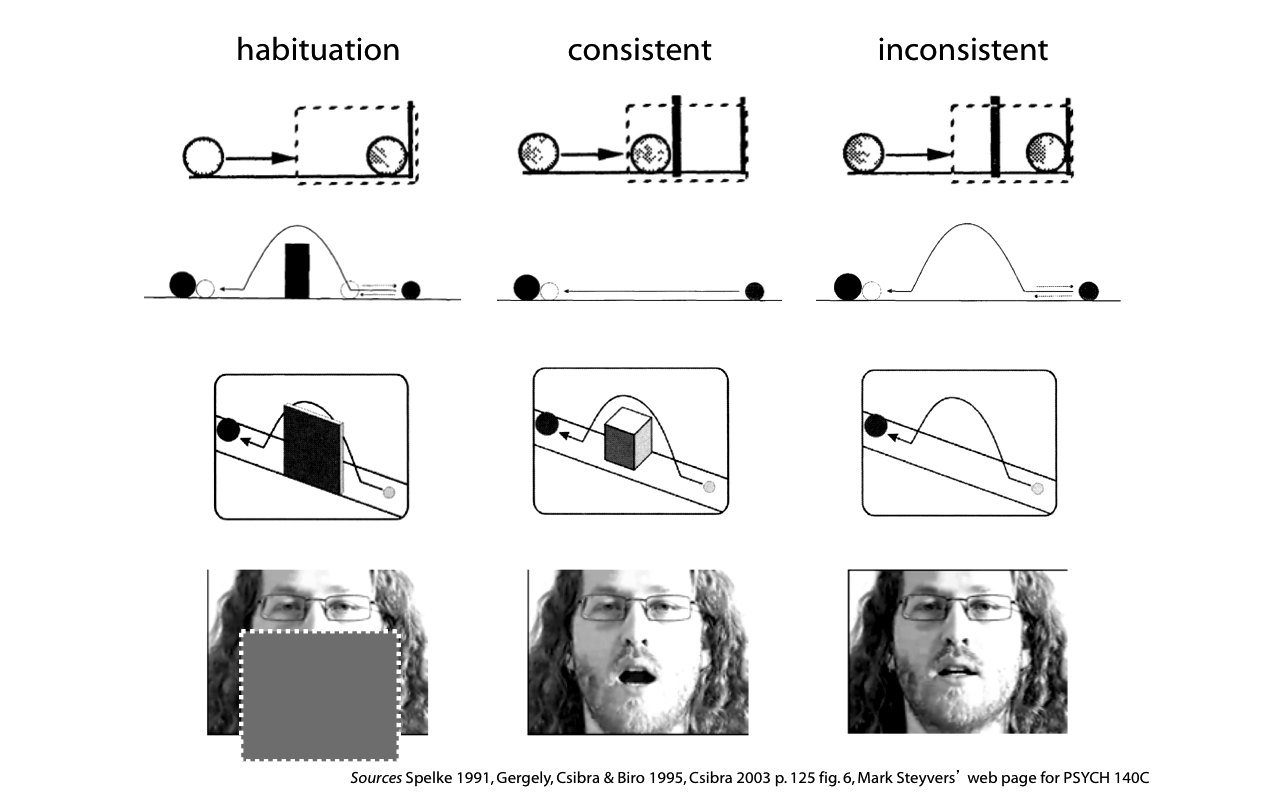
\includegraphics[width=0.3\textwidth]{fig1.png}
\end{center}


%‘Once they have learnt these terms [‘left’ and ‘blue’], the combinatorial machinery of natural language allows children to formulate and understand expressions such as left of the blue wall with no further learning’\citep{Spelke:2003fc} % (Spelke 2003: 296).

% 
%§4
%Four months: infants enjoy categorical perception of phonemes (Eimas, Siqueland, et al. 1971), which arguably involves a speech module (Liberman and Mattingly 1985).
%Three/four years: children first able to think and reason about phonemes as measured by standard tests for phonological awareness.
%Standard tests of phonological awareness:
%	- sorting according to initial phoneme
%	- phoneme segmentation, blending
%	- word completion
%	- … 
%Success on these tests is best explained by a single factor and: (i) depends on language spoken, (ii) depends on literacy and writing system, (iii) varies from phoneme to phoneme.
%‘it does not follow from the fact that a child can easily distinguish bud from bat that he can therefore respond analytically to the phonemic structure that underlies the distinction’ (I. Y. Liberman, Shankweiler, et al. 1974: 203). 



\footnotesize 
\bibliography{$HOME/endnote/phd_biblio}

\end{multicols}

\end{document}